% GNUPLOT: LaTeX picture with Postscript
\begingroup
  \makeatletter
  \providecommand\color[2][]{%
    \GenericError{(gnuplot) \space\space\space\@spaces}{%
      Package color not loaded in conjunction with
      terminal option `colourtext'%
    }{See the gnuplot documentation for explanation.%
    }{Either use 'blacktext' in gnuplot or load the package
      color.sty in LaTeX.}%
    \renewcommand\color[2][]{}%
  }%
  \providecommand\includegraphics[2][]{%
    \GenericError{(gnuplot) \space\space\space\@spaces}{%
      Package graphicx or graphics not loaded%
    }{See the gnuplot documentation for explanation.%
    }{The gnuplot epslatex terminal needs graphicx.sty or graphics.sty.}%
    \renewcommand\includegraphics[2][]{}%
  }%
  \providecommand\rotatebox[2]{#2}%
  \@ifundefined{ifGPcolor}{%
    \newif\ifGPcolor
    \GPcolorfalse
  }{}%
  \@ifundefined{ifGPblacktext}{%
    \newif\ifGPblacktext
    \GPblacktexttrue
  }{}%
  % define a \g@addto@macro without @ in the name:
  \let\gplgaddtomacro\g@addto@macro
  % define empty templates for all commands taking text:
  \gdef\gplbacktext{}%
  \gdef\gplfronttext{}%
  \makeatother
  \ifGPblacktext
    % no textcolor at all
    \def\colorrgb#1{}%
    \def\colorgray#1{}%
  \else
    % gray or color?
    \ifGPcolor
      \def\colorrgb#1{\color[rgb]{#1}}%
      \def\colorgray#1{\color[gray]{#1}}%
      \expandafter\def\csname LTw\endcsname{\color{white}}%
      \expandafter\def\csname LTb\endcsname{\color{black}}%
      \expandafter\def\csname LTa\endcsname{\color{black}}%
      \expandafter\def\csname LT0\endcsname{\color[rgb]{1,0,0}}%
      \expandafter\def\csname LT1\endcsname{\color[rgb]{0,1,0}}%
      \expandafter\def\csname LT2\endcsname{\color[rgb]{0,0,1}}%
      \expandafter\def\csname LT3\endcsname{\color[rgb]{1,0,1}}%
      \expandafter\def\csname LT4\endcsname{\color[rgb]{0,1,1}}%
      \expandafter\def\csname LT5\endcsname{\color[rgb]{1,1,0}}%
      \expandafter\def\csname LT6\endcsname{\color[rgb]{0,0,0}}%
      \expandafter\def\csname LT7\endcsname{\color[rgb]{1,0.3,0}}%
      \expandafter\def\csname LT8\endcsname{\color[rgb]{0.5,0.5,0.5}}%
    \else
      % gray
      \def\colorrgb#1{\color{black}}%
      \def\colorgray#1{\color[gray]{#1}}%
      \expandafter\def\csname LTw\endcsname{\color{white}}%
      \expandafter\def\csname LTb\endcsname{\color{black}}%
      \expandafter\def\csname LTa\endcsname{\color{black}}%
      \expandafter\def\csname LT0\endcsname{\color{black}}%
      \expandafter\def\csname LT1\endcsname{\color{black}}%
      \expandafter\def\csname LT2\endcsname{\color{black}}%
      \expandafter\def\csname LT3\endcsname{\color{black}}%
      \expandafter\def\csname LT4\endcsname{\color{black}}%
      \expandafter\def\csname LT5\endcsname{\color{black}}%
      \expandafter\def\csname LT6\endcsname{\color{black}}%
      \expandafter\def\csname LT7\endcsname{\color{black}}%
      \expandafter\def\csname LT8\endcsname{\color{black}}%
    \fi
  \fi
  \setlength{\unitlength}{0.0500bp}%
  \begin{picture}(7300.00,2520.00)%


      \put(846,2700){\makebox(0,0)[r]{\strut{} \textbf{A}}}%


      \put(946,704){\makebox(0,0)[r]{\strut{} 0}}%
      \put(946,1092){\makebox(0,0)[r]{\strut{} 0.2}}%
      \put(946,1480){\makebox(0,0)[r]{\strut{} 0.4}}%
      \put(946,1868){\makebox(0,0)[r]{\strut{} 0.6}}%
      \put(946,2256){\makebox(0,0)[r]{\strut{} 0.8}}%
      \put(1582,484){\makebox(0,0){\strut{} 150}}%
      \put(2122,484){\makebox(0,0){\strut{} 300}}%
      \put(2663,484){\makebox(0,0){\strut{} 450}}%
      \put(3203,484){\makebox(0,0){\strut{} 600}}%
      \put(176,1480){\rotatebox{-270}{\makebox(0,0){\strut{}mutual information (bits)}}}%
      \put(2140,154){\makebox(0,0){\strut{}$h$}}%


      \put(4546,2700){\makebox(0,0)[r]{\strut{} \textbf{B}}}%

      \put(4646,704){\makebox(0,0)[r]{\strut{} 0}}%
      \put(4646,1014){\makebox(0,0)[r]{\strut{} 50}}%
      \put(4646,1325){\makebox(0,0)[r]{\strut{} 100}}%
      \put(4646,1635){\makebox(0,0)[r]{\strut{} 150}}%
      \put(4646,1946){\makebox(0,0)[r]{\strut{} 200}}%
      \put(4646,2256){\makebox(0,0)[r]{\strut{} 250}}%
      \put(5289,484){\makebox(0,0){\strut{} 100}}%
      \put(5827,484){\makebox(0,0){\strut{} 200}}%
      \put(6365,484){\makebox(0,0){\strut{} 300}}%
      \put(6903,484){\makebox(0,0){\strut{} 400}}%
      \put(3876,1480){\rotatebox{-270}{\makebox(0,0){\strut{}$h$}}}%
      \put(5840,154){\makebox(0,0){\strut{}spike train length (s)}}%

    \put(3700,0){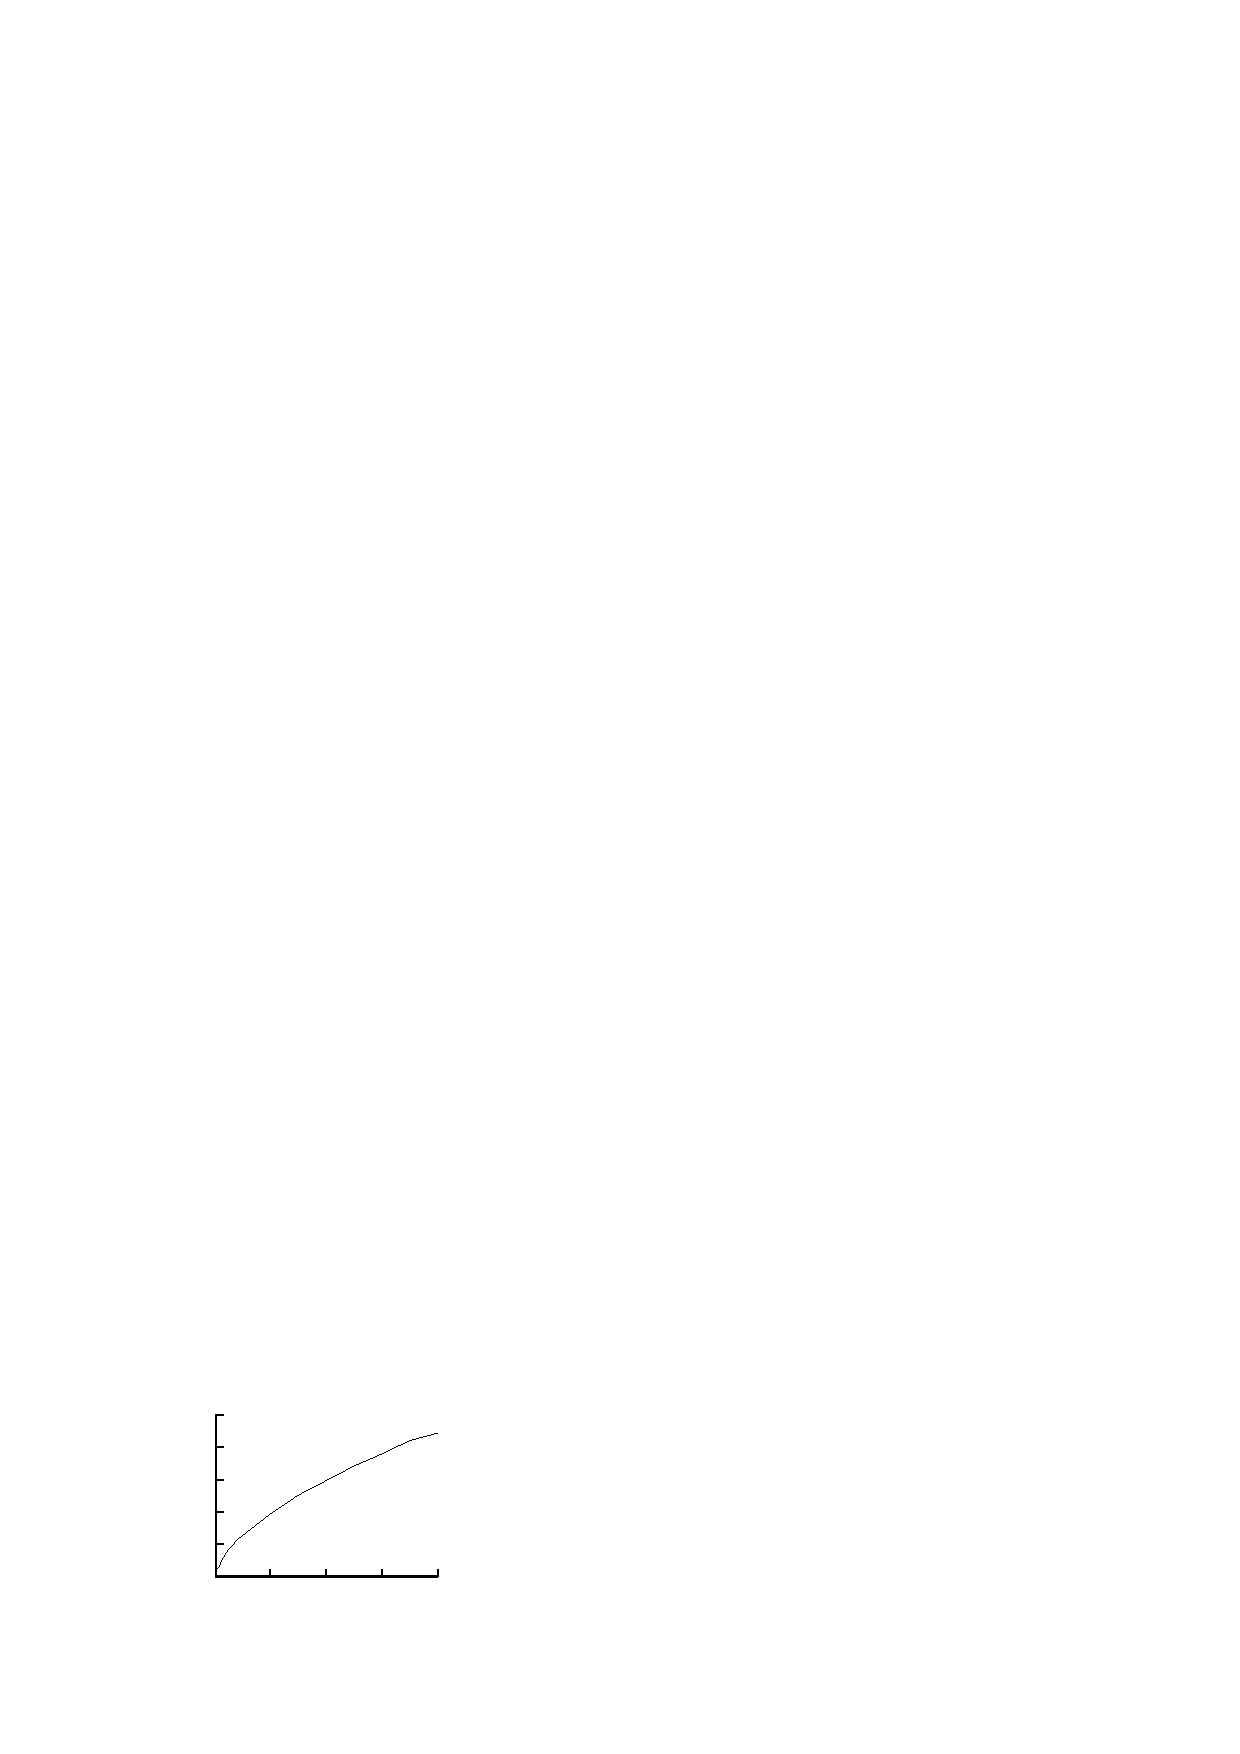
\includegraphics{fig_best_h}}
    \put(0,0){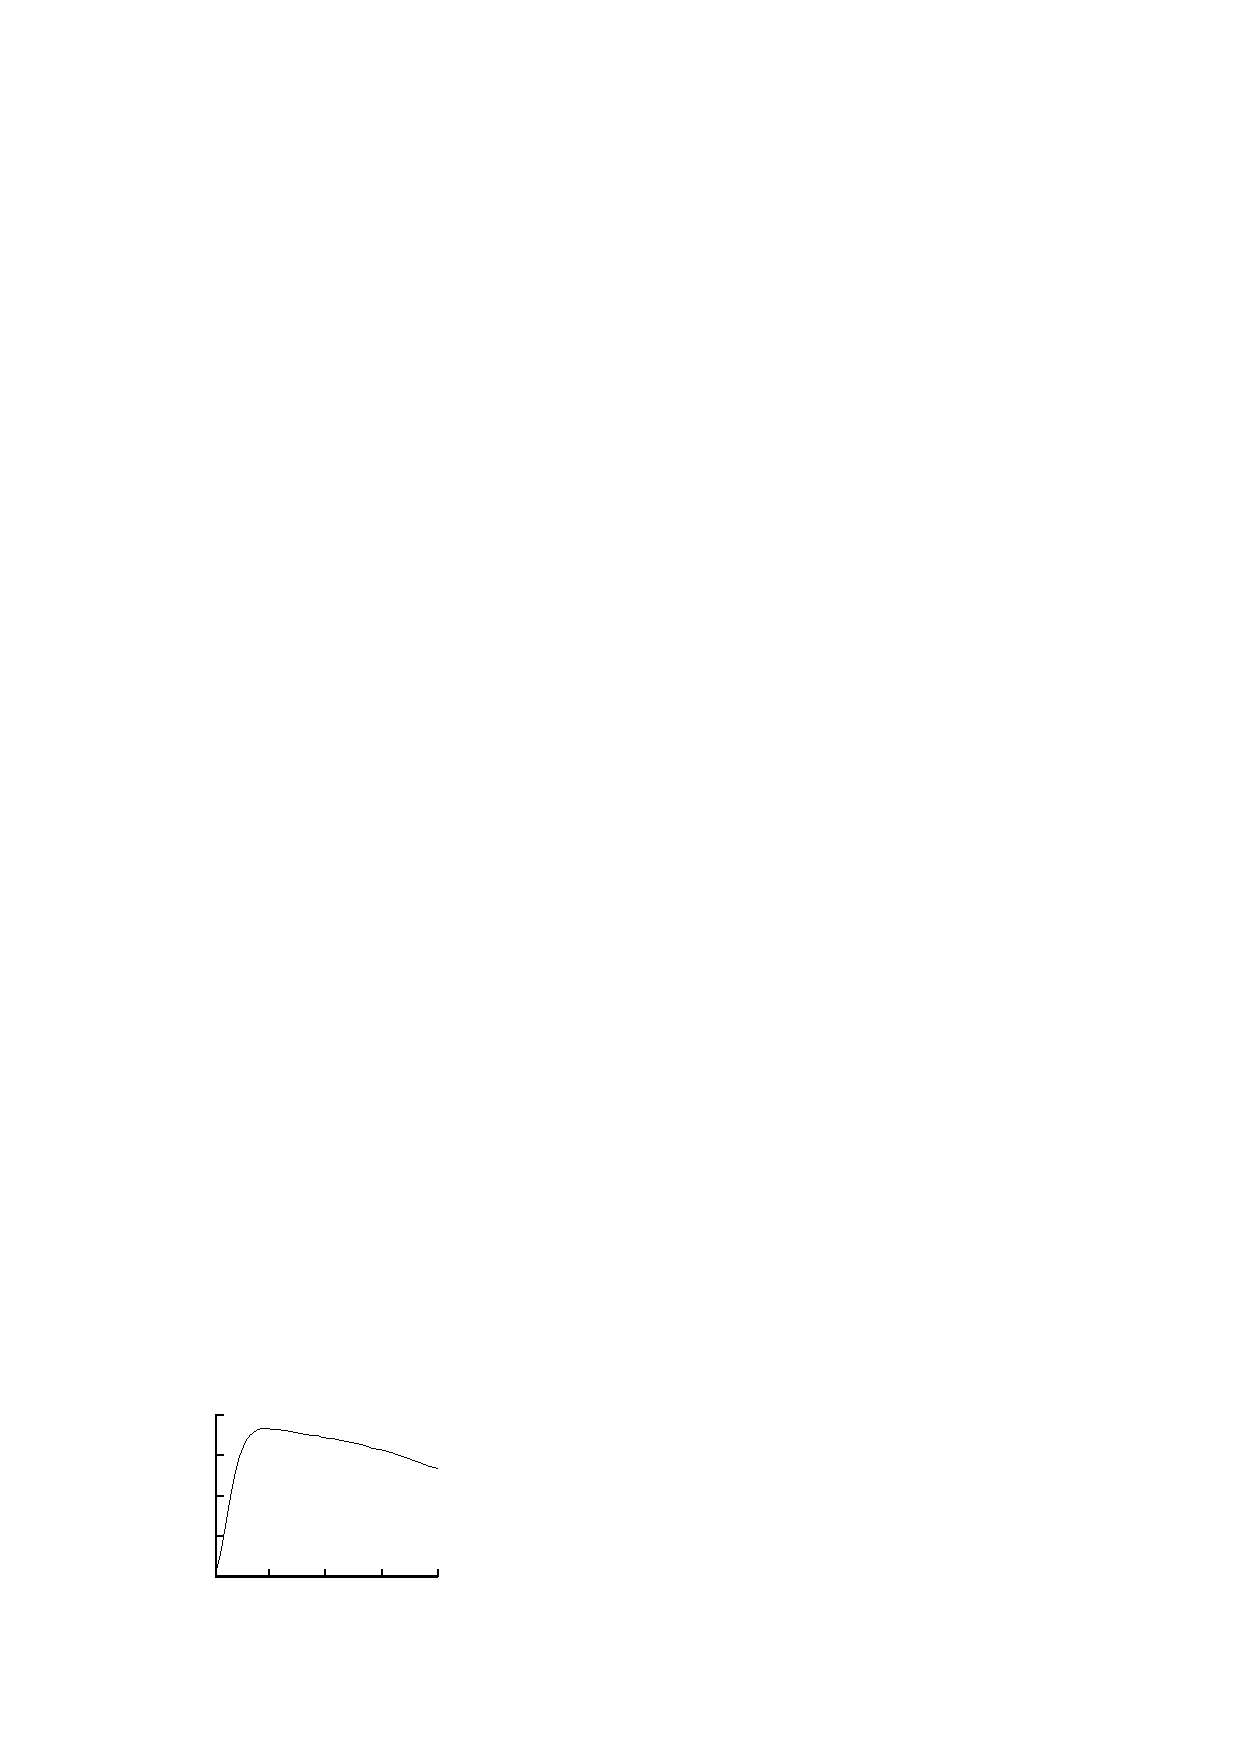
\includegraphics{fig_h_sweep}}%

  \end{picture}%
\endgroup
